\section{Theorie}
\label{sec:Theorie}

\subsection{Fehlerrechnung}

Für die Fehlerfortpflanzung bei Gleichungen mit $N$ fehlerbehafteten Größen
wird jeweils die Formel zur Gaußschen Fehlerfortpflanzung

\begin{equation*}
  \sigma = \sqrt{\sum_{i=1}^{N}\biggl(\frac{\partial f(x_{\g{i}})}{\partial x_{\g{i}}}
  \sigma_{\g{i}}\biggr)^2}
\end{equation*}
mit der jeweiligen Funktion $f(x_{\g{i}})$, den Messgrößen $x_{\g{i}}$ und den
zugehörigen Fehlern $\sigma_i$ verwendet.
Zur Berechnung des arithmetischen Mittels von $N$ Messwerten wird jeweils die
Formel

\begin{equation*}
  \bar{x} = \frac{1}{N}\sum_{i=1}^{N}x_{\g{i}}
\end{equation*}
mit den Messwerten $x_i$ benutzt.
Die Standardabweichung des Mittelwerts wird jeweils mit der Gleichung

\begin{equation*}
  \bar{\sigma} = \sqrt{\frac{1}{N-1}\sum_{i=1}^{N}(x_{\g{i}} - \bar{x})^2}
\end{equation*}
mit den $N$ Messwerten $x_i$ berechnet.

\subsection{Einleitung}

Lichtbeugung tritt im Allgemeinen auf, wenn der Strahldurchmesser eines
einfallenden Lichtstrahls größer als die Abmessungen des Beugungsobjektes sind.
Das Licht kann in diesem Fall als Welle genähert werden und es enstehen
Interferenzen hinter dem Beugungsobjekt.
Im folgenden Versuch soll die Abhägigkeit des Interferenzmusters von der
Aperturfunktion, also der Gestalt des Beugungsobjektes, untersucht werden.
Bei der allgemeinen Lichtbeugung wird zwischen der Fresnelschen und der
Fraunhoferschen Beugung unterschieden. Diese Fälle sind in Abbildung
\ref{fig:fraunfresnel} für die Beugung an einem Einzelspalt dargestellt.

\begin{figure}
  \centering
  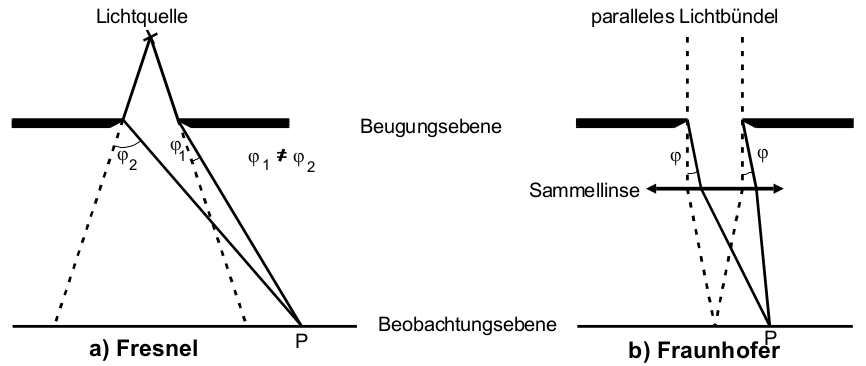
\includegraphics[height=5cm]{MeinePics/fraunfresnel.png}
  \caption{Fresnelsche und Fraunhofersche Lichtbeugung am Einzelspalt. Die
  gestrichelten Linien beschreiben den theoretischen Strahlenverlauf in der
  geometrischen Optik.\cite{anleitung}}
  \label{fig:fraunfresnel}
\end{figure}

\FloatBarrier

Bei der Fresnelschen Beugung ist die Entfernung der Lichtquelle vom Spalt
nicht deutlich größer als der Spalt. Dadurch interferieren hinter dem Spalt
Lichtstrahlen, die mit unterschiedlichen Winkeln abgelenkt wurden.
Bei der Fraunhoferschen Beugung ist der Abstand zwischen Lichtquelle und Spalt
viel größer als die Spaltbreite, sodass die am Spalt eintreffenden
Lichtstrahlen annähernd parallel sind. Hinter dem Spalt interferieren
bei dieser Beugung nur Strahlen, die mit dem selben Winkel abgelenkt wurden.
In diesem Versuch werden nur Beugungsmuster einer Fraunhoferschen
Lichtbeugung betrachtet, da diese mathematisch einfacher zu behandeln sind.


\subsection{Beugung am Einzelspalt}

Beim Einzelspalt ist die Höhe des Spalts viel größer als die Breite $b$, sodass
nur die Beugung in $x$-Richtung, also in Richtung Spaltbreite, betrachtet
werden muss.
Fällt eine ebene Welle, zum Beispiel ein Laser, mit der Feldstärke
\begin{align}
  A(z,t) = A_0 \symup{e}^{i(\omega t - \frac{2\pi z}{\lambda})}
\end{align}
ein, so wird diese am Spalt gebeugt. Das Huygensche Prinzip besagt, dass
an jedem Punkt im Spalt Kugelwellen ausgesendet werden, die dann hinter dem
Spalt interferieren und eine neue Wellenfront bilden. Diese ist nicht nur,
wie in der geometrischen Optik auf den Bereich hinter der Spaltöffnung begrenzt,
sondern auf den gesamten Bereich hinter dem Beugungsobjekt.
In Abbildung \ref{fig:phasenbeziehung} ist eine Skizze zur Bestimmung des
Phasenunterschiedes zwischen zwei mit gleichem Winkel abgelenkten Strahlen
abgebildet.

\begin{figure}
  \centering
  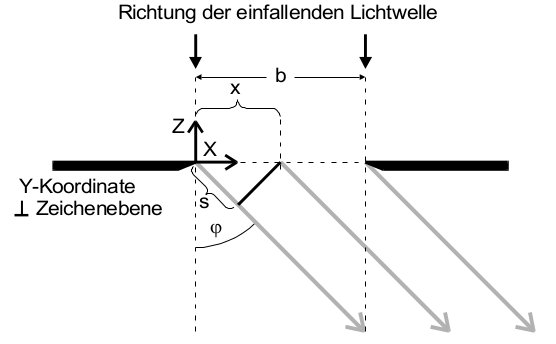
\includegraphics[height=5cm]{MeinePics/phasenbeziehung.png}
  \caption{Skizze zur Bestimmung der Phasendifferenz zwischen zwei Strahlen,
  die an unterschiedlichen Stellen mit jeweils dem selben Winkel abgelenkt
  werden.\cite{anleitung}}
  \label{fig:phasenbeziehung}
\end{figure}

\FloatBarrier

Für die Phasendifferenz ergibt sich
\begin{align}
  \delta = \frac{2 \pi x \sin{\varphi}}{\lambda}.
\end{align}
Nach Integration über die Spaltbreite und einigen Umformungsschritten folgt
die Amplitude hinter dem Spalt
\begin{align}
  B(z,t,\varphi) = A_0 b \symup{e}^{\symup{i}(\omega t - \frac{2 \pi z}{\lambda})}
  \symup{e}^{\frac{\pi \symup{i} b \sin{\varphi}}{\lambda}}
  \text{sinc}\Bigl(\frac{\pi \sin{\varphi}}{\lambda}\Bigr).
  \label{eqn:amplitudeeinzel}
\end{align}
Da die Exponentialfunktionen in \eqref{eqn:amplitudeeinzel} nur
Phasenverschiebungen sind, lässt sich die Amplitude auch darstellen als
\begin{align}
  B(\varphi) = A_0 b \text{  sinc}(\eta)
  \label{eqn:sinc}
\end{align}
mit
\begin{align}
  \eta(\varphi) = \frac{\pi b \sin{\varphi}}{\lambda}.
  \label{eqn:eta}
\end{align}
Die Amplituden-Funktion ist in Abbildung \ref{fig:sincf} dargestellt.

\begin{figure}
  \centering
  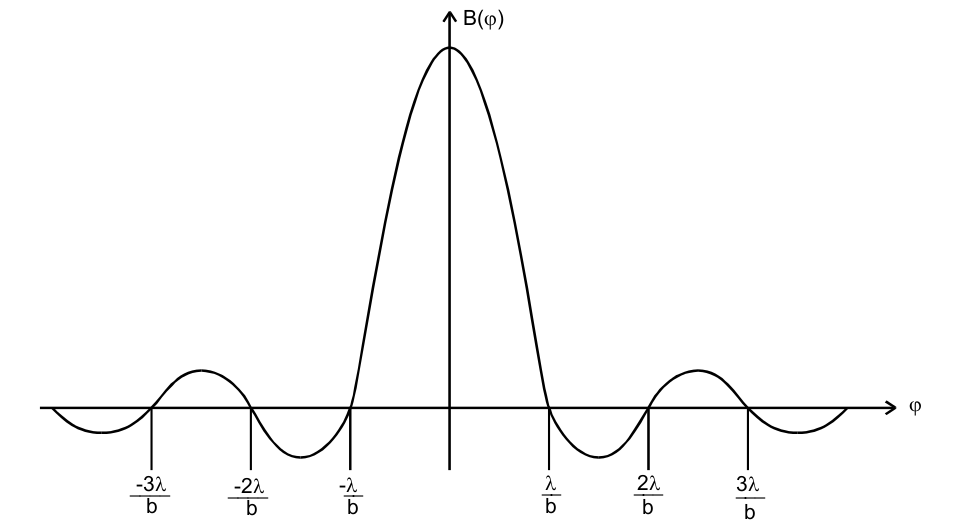
\includegraphics[height=7cm]{MeinePics/sinc.png}
  \caption{Skizze der Amplituden-Funktion \eqref{eqn:sinc}.\cite{anleitung}}
  \label{fig:sincf}
\end{figure}

\FloatBarrier

Die Nullstellen liegen bei
\begin{align}
  \sin{\varphi_n} = \pm n \frac{\lambda}{b}
  \label{eqn:nullstelleneinzel}
\end{align}
mit natürlichem $n$.
Die Amplituden-Funktion kann aufgrund hoher Frequenzen nicht gemessen werden,
stattdessen misst man die Lichtintensität an einem Schirm.
Die Intensitätsfunktion entspricht dem Betragsquadrat der Amplitudenfunktion
und ist daher an jedem Ort positiv.
Sie lautet mit \eqref{eqn:eta}
\begin{align}
  I(\varphi) = A_0^2 b^2 \text{sinc}^2(\eta)
  \label{eqn:intensitaeteinzel}
\end{align}


\subsection{Beugung am Doppelspalt}

Die Intensitätsverteilung bei der Beugung am Doppelspalt lässt sich ähnlich
wie die am Einzelspalt berechnen.
Eine Skizze hierzu ist in Abbildung \ref{fig:doppelspalt} dargestellt.

\begin{figure}
  \centering
  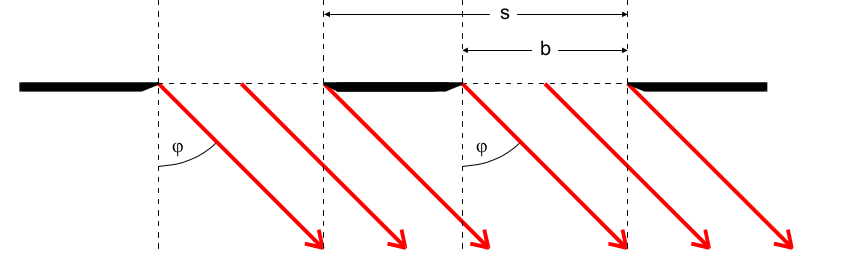
\includegraphics[height=3.5cm]{MeinePics/doppelspalt.png}
  \caption{Beugung am Doppelspalt.\cite{anleitung}}
  \label{fig:doppelspalt}
\end{figure}

\FloatBarrier

Aus der Überlagerung zweier Einzelspalte folgt die Intensität am Doppelspalt
\begin{align}
  I(\varphi) = 4 \cos^2{\frac{\pi s \sin{\varphi}}{\lambda}}
  \text{sinc}^2\Bigl(\frac{\pi b \sin{\varphi}}{\lambda}\Bigr).
  \label{eqn:intensdoppel}
\end{align}
Durch den Cosinus-Faktor enthält die Funktion zusätzlich zu den Nullstellen
\eqref{eqn:nullstelleneinzel} noch an den Stellen
\begin{align}
  \varphi_k = \lambda \arcsin{\frac{2k+1}{2s}}
\end{align}
mit natürlichem $k$ weitere Nullstellen.


\subsection{Beugungsobjekt und Fouriertransformation}

Die Fraunhofer-Näherung besagt, dass die Amplitudenverteilung die
Fouriertransformierte der Aperturfunktion ist.
Das heißt, dass für die Intensitätsverteilung einer beliebigen
Beugungsfunktion $f(x)$
\begin{align}
  I(p) = \lvert \int_{-\infty}^{\infty} f(x) \symup{e}^{\symup{i}px} \symup{d}x
  \rvert^2
\end{align}
gilt.
Die Intensitätsfunktion am Einzelspalt \eqref{eqn:intensitaeteinzel}
folgt somit auch aus der Aperturfunktion
\begin{align}
  f(x) =
  \begin{cases}
    A_0, & \text{für  } 0 \leq x \leq b \\
    0, & \text{sonst}
  \end{cases}
\end{align}
mit
\begin{align}
  p = \frac{2 \pi \sin{\varphi}}{\lambda}.
\end{align}
